\documentclass[11pt]{article}
\usepackage{icmlko}
\begin{document}

\title{이득은 옛것이라서가 아니라 아래라서였다 --- 835편을 시대로 갈라 보니}
\author{월드모델 실험실}
\date{노트 388 · 2026년 8월 1일}
\maketitle

\begin{abstract}
노트 387이 웹툰 아카이브 835편(2005\,--\,2020)을 학습에 더해 판을
$0.4355 \to 0.4423$ 으로 올렸고, 위약(새 행 라벨 섞기)이 그 이득을 통째로
지우는 것을 보였다 --- \emph{행이 많아서가 아니라 그 라벨이 말하는 것}
때문이다. 그런데 \emph{무엇이} 말하는지는 ``관측으로 둔다''고 적고 넘겼다.
갈랐다.

835편을 시대 셋으로 나눠 각각만 더해 봤다. 개수가 거의 같아
(292 · 292 · 251) 행 수가 교락하지 않는다.

\begin{center}
\begin{tabular}{lrrrrr}
\hline
시대 & 행 & 판 차 & 부호 & 웹툰 차 & 부호 \\
\hline
E1 2005\,--\,2012 & 292 & $\mathbf{+0.0063}$ & \textbf{10/12} & $+0.0199$ & 8/12 \\
E2 2013\,--\,2016 & 292 & $+0.0007$ & 7/12 & $+0.0000$ & 5/12 \\
E3 2017\,--\,2020 & 251 & $+0.0025$ & 8/12 & $+0.0087$ & 8/12 \\
\hline
전부 (노트 387) & 835 & $+0.0071$ & 11/12 & $+0.0305$ & 12/12 \\
\hline
\end{tabular}
\end{center}

\textbf{제일 오래된 292편이 전체 이득의 89\%를 낸다.} E1 혼자서도 부호가
10/12 라 노트 378 조항 ①로 채택될 값이고, E2는 판 차가 $+0.0007$ ·
웹툰 차가 정확히 $+0.0000$ 이다.

\textbf{그런데 시대가 원인이 아니다.} 세 무리의 라벨을 보면 E1만 다르다:

\begin{center}
\begin{tabular}{lrrrr}
\hline
 & 라벨 퍼짐 & 최소 & 옛 학습 최소 아래 & 옛 1분위 아래 \\
\hline
E1 & \textbf{1.019} & \textbf{1.954} & \textbf{29편 (10\%)} & 151편 (52\%) \\
E2 & 0.513 & 3.402 & 0 & 65편 (22\%) \\
E3 & 0.546 & 3.058 & 0 & 76편 (30\%) \\
\hline
\end{tabular}
\end{center}

기존 학습 2,106행의 라벨 최소가 2.612 인데 \textbf{E1만 그 아래로
내려간다}(29편) --- E2 · E3는 한 편도 없다. 퍼짐도 E1이 둘의 두 배다.
\textbf{이득의 출처는 ``옛 작품''이 아니라 ``학습 라벨 범위를 아래로
넓힌 것''이다.}

이것이 이번 사이클 전체를 하나로 묶는다. 노트 376은 세계애니를 아래로
못 넓혔고(그 구간에 신호가 없다), 노트 385\,--\,386은 그 가부가 도메인마다
갈린다는 것을 넷으로 확인했다. \textbf{웹툰은 넓힐 수 있는 쪽이었고, 넓히니
판이 올랐다.}
\end{abstract}

\section{설계 --- 개수를 맞춘다}

노트 387의 결론은 ``라벨이 말하는 것''까지였고 무엇이 말하는지는 안 갈랐다.
후보가 셋 있었다 --- 시대가 넓어진 것 · 완결작이라 축이 사후가 아닌 것 ·
라벨 범위가 아래로 넓어진 것.

시대로 가르면 셋을 어느 정도 분리할 수 있다. 835편의 연도 분포가 마침
셋으로 거의 균등하게 나뉜다(292 · 292 · 251)라 \textbf{행 수가 교락하지
않는다} --- 노트 259가 ``자리가 모자라서''를 잡음 열로 반증한 것과 같은
자리다. 완결 비율은 셋 다 99\,--\,100\% 라 두 번째 후보도 상수가 된다.

채택 전 챔피언을 A로 두고 각 시대만 더한 세 팔을 만들어 짝 12뽑기로
견줬다. 유보 711행은 네 팔이 전부 같다(노트 378 조항 ④).

\begin{figure}[t]
\centering
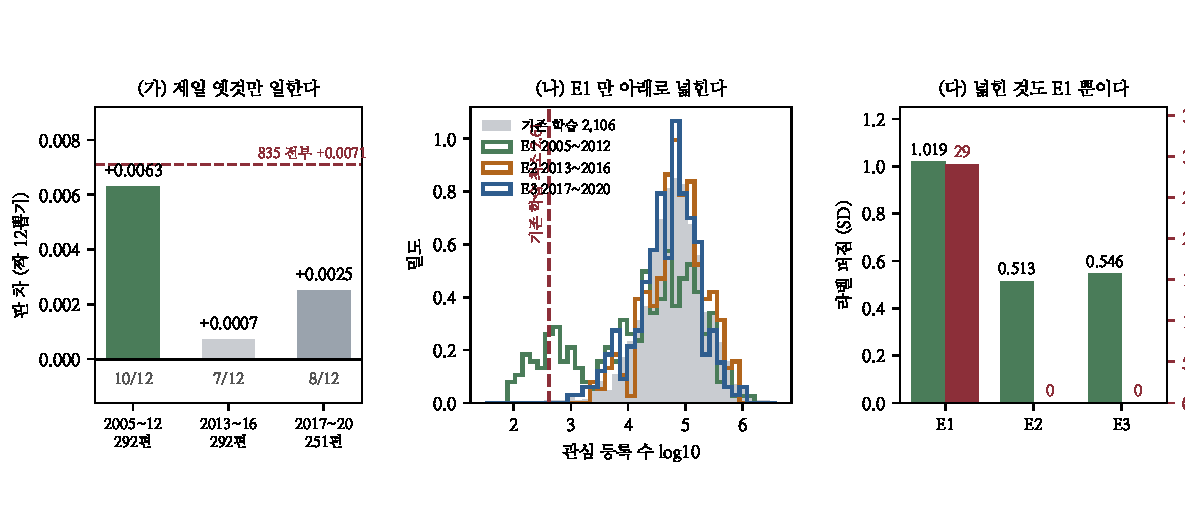
\includegraphics[width=\linewidth]{figs/fig388.pdf}
\caption{\textbf{(가)} 시대별 판 차. 제일 옛것(E1)이 전체 $+0.0071$ 의
89\%를 낸다. \textbf{(나)} 기존 학습 라벨 분포(회색)와 세 시대. 붉은 선은
기존 학습의 최소($2.612$)이고 \textbf{E1만 그 왼쪽에 꼬리가 있다}.
\textbf{(다)} 라벨 퍼짐과 옛 최소보다 낮은 행 수 --- 둘 다 E1만 다르다.}
\label{fig:main}
\end{figure}

\section{시대가 아니라 범위다}

E1이 이겼다고 ``옛 작품이 좋다''로 읽으면 안 된다. E1이 다른 것은 시대만이
아니다.

\textbf{E1의 라벨 퍼짐이 1.019 로 E2(0.513) · E3(0.546)의 두 배다.} 2005년
전후의 웹툰은 관심 수가 90(=$10^{1.954}$)짜리부터 백만대까지 있는데,
2013년 이후는 다들 수천\,--\,수십만 안에 모여 있다. 플랫폼이 커지면서
아래쪽이 사라진 것이다.

\textbf{그리고 E1만 기존 학습의 아래를 넘어간다.} 기존 학습 2,106행의 최소가
$10^{2.612}\approx410$ 인데 E1에는 그보다 낮은 것이 29편, 기존 1분위
($\approx3$만) 아래가 151편(52\%)이다. E2 · E3는 기존 최소 아래가
\textbf{0편}이다.

\textbf{그러니 세 후보 중 살아남는 것은 셋째다} --- 학습 라벨 범위를 아래로
넓혔다. 첫째(시대)와 E1은 붙어 있어서 완전히는 못 가르지만, E2와 E3가
서로 다른 시대인데 둘 다 이득이 없다는 것이 시대 자체는 아니라는 쪽을
가리킨다.

\textbf{안 갈린 것도 적는다.} ``퍼짐이 넓어서''와 ``아래로 갔기 때문''은
E1 안에서 같이 움직이므로 이 실험으로 못 가른다. 가르려면 E1에서 위쪽만
잘라 퍼짐만 좁힌 팔이 필요한데, 노트 386이 배운 대로 잘라서 좁히면 그
자체가 다른 것을 바꾼다.

\section{이번 사이클이 하나로 묶인다}

\begin{center}
\begin{tabular}{lll}
\hline
도메인 & 아래로 넓힐 수 있나 & 결과 \\
\hline
세계애니 (376) & 아니다 (아래 $\rho\,{+}0.0223$) & 안 넓혔다 \\
펀딩 (379 · 381) & 아니다 (아래 $\rho\,{-}0.0094$) & 채점을 고치니 $-$, 학습을 고치니 $+0.0322$ \\
게임 (385) & 그렇다 ($+0.2746$) & 애초에 안 부풀어 있었다 \\
만화 (386) & 그렇다 ($+0.1046$, 59\%ile) & 안 부풀어 있었다 \\
\textbf{웹툰} (387 · 388) & \textbf{그렇다} & \textbf{넓히니 판 $+0.0071$} \\
\hline
\end{tabular}
\end{center}

노트 385가 ``부풀리는 것은 잘려 나간 구간에서 축이 안 통할 때다''로
고친 규칙은 \emph{점수를 읽는 법}이었는데, 여기서 \emph{무엇을 모을지}로도
쓰인다 --- \textbf{아래에서 축이 통하는 도메인은 아래를 모으면 이득이
난다.} 웹툰이 그 첫 사례다.

\section{남은 것}

\begin{center}
\begin{tabular}{lll}
\hline
항목 & 왜 값이 큰가 & 어떻게 \\
\hline
애니 아카이브 & 무게 606 · 덮음 22\% · 같은 모양 & 수집 중(3,000 목표) \\
웹툰 더 아래 & E1 이 통했으니 더 아래도 & 플랫폼에 그보다 아래가 없다 \\
퍼짐 대 범위 & E1 안에서 안 갈렸다 & 다른 도메인에서 갈라 본다 \\
웹툰 나머지 175편 & 덮음 95\% $\to$ 100\% & 수집이 멈췄다 \\
\hline
\end{tabular}
\end{center}

\end{document}
